\section{Introduction}

Many systems -- from supercomputer installations to embedded
systems-on-chip -- benefit from using special-purpose
{\em accelerators} which can significantly outperform general-purpose
processors in terms of energy efficiency as well as
execution speed.
Software for such systems, however, is currently written using
low-level APIs \nomenclature{APIs}{Application Program Interface},
such as OpenCL (Open Computing Language)\nomenclature{OpenCL}{Open Computing Language}~\cite{stoneopencl} and
CUDA (Compute Unified Device Architecture)\nomenclature{CUDA}{Compute Unified Device Architecture}~\cite{cudaref},
which increases the cost of
its development and maintenance.
A compelling alternative for developers is to work with higher-level
programming languages, and to leverage compilation technology to automatically
generate efficient low level code.

For general-purpose languages in the C family, this approach is hindered
by the difficulty of static analysis in the presence of pointer aliasing.
The possibility of aliasing often forces a parallelizing compiler
to assume that it is \emph{not} safe to parallelize a region of source
code, even though aliasing might not actually
occur at runtime.

Domain-specific languages (DSLs) can circumvent this problem: it is often
clear how parallelism can be exploited given
high-level knowledge about standard operations in a given domain, such as
linear algebra~\cite{vobla2014},
image processing~\cite{DBLP:conf/pldi/Ragan-KelleyBAPDA13}
or partial differential equations~\cite{DBLP:journals/toms/AlnaesLORW14}.
The drawback of the DSL approach is the significant effort required to
lower code all the way from the DSL level to highly optimized OpenCL or CUDA.
The effort involved is even more significant if optimization is required
for multiple platforms.
Given typical budget constraints, the DSL implementers will
likely limit their efforts to a set of techniques useful for a small
number of target platforms, thus
compromising on performance portability.  Moreover, the implementers
of different DSLs will likely spend their efforts on implementing an
overlapping set of techniques.
The existence of a common intermediate language serving as a target
for DSL compilers would reduce considerably the development costs.

% To some extent, the design of such an intermediate
% language obeys the same motivations that led to the design of compiler
% middle-ends that support a common set of analyses and optimizations
% for a variety of programming languages and target instruction
% sets. However, the technical context is very different, involving
% code generation for complex memory hierarchies and massively parallel
% hardware accelerators. This involves program analyses and
% transformations on multidimensional iteration spaces and arrays,
% dealing with mapping, scheduling, and automatic data transfers in a
% massively concurrent context.
% 
% Beside enhancing productivity, DSLs have the advantage of using high level
% constructs that have rich semantics.  These constructs provide a wealth of
% information that enable the compiler to optimize and parallelize
% the code even for algorithms that are considered to be irregular
% when expressed in languages like C (e.g., operations on lists, like map).
% %
% DSL compilers maintain tight control over the generated code, eliminating
% many of the problems faced by general-purpose optimizing compilers.

We present the design and implementation of \pencil, a plat\-form-neu\-tral 
compute intermediate language.
\pencil aims to serve both as a portable implementation language to facilitate 
the acceleration of new and legacy applications on modern accelerators, and as 
a tractable target language for DSL compilers.


\section{\pencil Language}

\subsection{Overview of PENCIL \label{pencil-overview}}

\pencil is a rigorously-defined subset of C99~\cite{c99}
\nomenclature{C99}{C Standard 1999}.  It enforces a set of
coding rules principally related to restricting the manner in which pointers
can be manipulated.  These restrictions make \pencil code
``static analysis-friendly'': the rules are designed to enable a compiler
to perform better optimization and parallelization when translating \pencil
to a lower-level formalism such as OpenCL.
\pencil is also equipped with specific language constructs, including
\emph{assume predicates} and \emph{side effect summaries} for functions,
that enable communication of domain-specific information and static properties
to the \pencil compiler, to be used for parallelization and optimization.
These specific constructs provide information that is difficult for a
compiler to extract from arbitrary code but that can be easily captured from a DSL, or
expressed by an expert programmer.
Although the target platforms are highly parallel,
\pencil deliberately has sequential C99 semantics in order to simplify DSL
compiler development and the work of a domain expert directly
developing in \pencil, and more importantly, to avoid committing to
any particular pattern(s) of parallelism.

Where necessary, \pencil exploits the flexibility of non-C99 GNU
C extensions~\cite{gccguide} such as type attributes, and exploits
pragmas when no alternative is available.
The latter have been inspired from standard pragmas used as annotations
for vectorization and thread-level parallelism, but retain a strictly
sequential semantics in \pencil.

A design goal was to avoid pragma-based directives as directives are still
not considered to be first class citizens by many compilers.
However, in very few cases, \pencil relies on a directive to attach
properties to a control flow region of the code, no better C-compatible
alternative being available.

Because it is based on C, the learning curve for \pencil is gentle.
By design, \pencil interfaces with non-\pencil C code, so that legacy C 
applications can be
incrementally ported into \pencil.  From the point of view of DSL
compilation, \pencil offers a tractable target because all a DSL-to-\pencil
compiler must do is faithfully encode the semantics of the input DSL program
into \pencil; auto-parallelization and optimization for multiple accelerator
targets is then taken care of by the downstream compiler.
Because DSL-to-\pencil compilers have tight control over the code they
generate, such compilers can aid the effectiveness of the downstream
\pencil compiler by careful generation of code, and by communicating
domain-specific information via the language constructs \pencil provides
for this purpose.


\paragraph*{Design considerations}
The design of \pencil is guided by the following considerations:
\begin{itemize}
\item \pencil should have sequential semantics to facilitate the
  design and implementation of domain-specific compilers targeting
  \pencil, to ease the work of \pencil programmers, and to avoid committing
  early on target-specific patterns of parallelism.
  Besides that, this allows any C99 compiler that supports GNU C99 extensions
  to provide a reference implementation for \pencil.

\item \pencil should simplify static code analysis for the optimizing compiler.
  For example, the use of pointers is disallowed, except in specific cases,
  relieving the compiler from issues related to aliasing.

\item \pencil should provide facilities that allow a DSL-to-\pencil
  compiler to convey, in the \pencil code that it generates,
  domain-specific information that can be exploited by the
  compiler to perform better optimizations.  For example, \pencil
  should allow the user to indicate that the size of an array does not
  exceed a specific size to enable the compiler to place
  that array in the shared memory of a GPU (Graphics Processing Unit).

\item For compatibility reasons, a standard C99 compiler that supports
  GNU C attributes~\cite{gccguide} should be able to compile \pencil, this allows for
  greater portability and makes the debugging of \pencil code easier.

\item The subset of C99 that constitutes \pencil should
  be as large as the above design  considerations permit.
  A very small and restrictive subset limits the reuse and
  modularity of \pencil code, and makes
  \pencil less attractive to programmers and
  DSL compiler-writers.

\item Language extensions (compared to C99) should be minimized.
  Too many extensions make it harder for compilers
  to support \pencil.

\item \pencil code should be able to interface with non-\pencil code
  and external library functions.
\end{itemize}

Three possible scenarios of using \pencil are possible:
\begin{enumerate}
\item \pencil code is generated by a DSL compiler;
\item \pencil code is written by an expert programmer;
\item a mixture of both scenarios.
\end{enumerate}

\begin{figure}[ht]
{
 \centering
 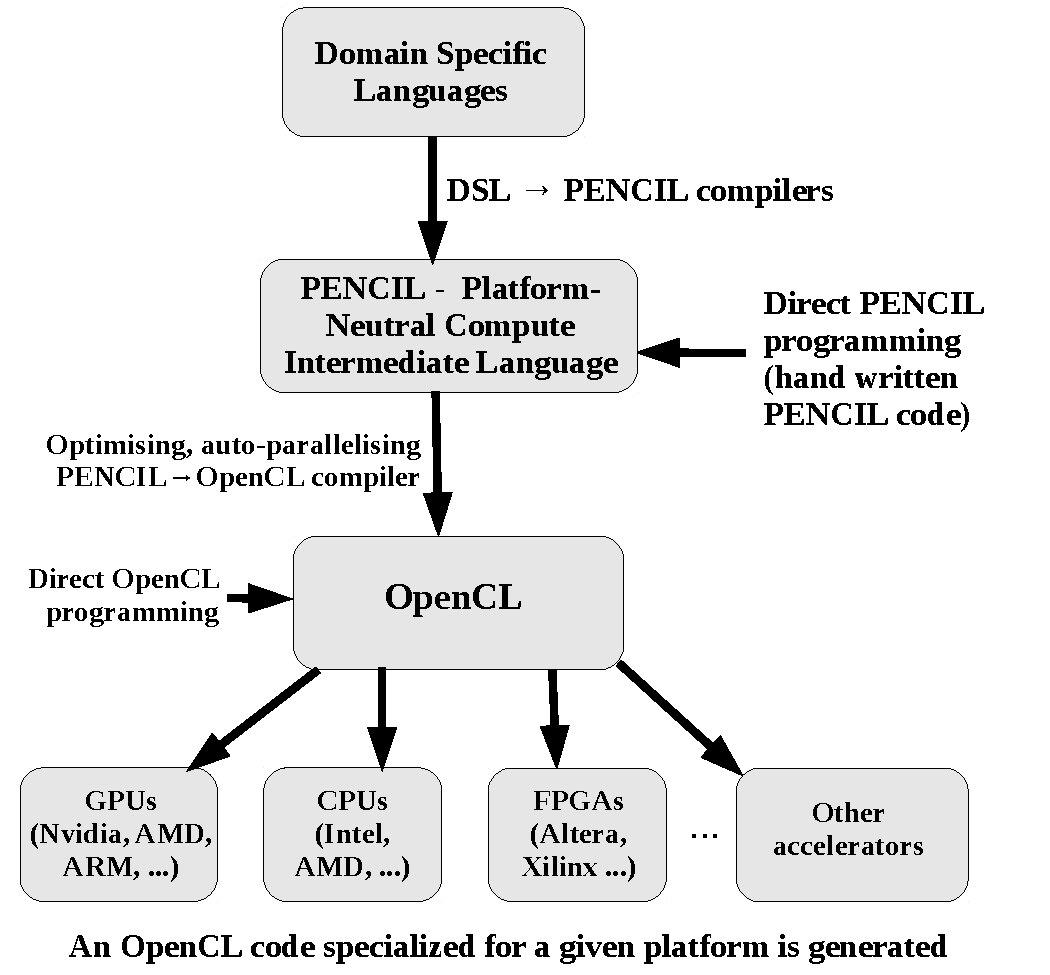
\includegraphics[scale=0.65]{./figures/CARPHighLevelOverview.pdf}
 \caption{High level overview of our vision for the use of PENCIL}
 \label{fig-pencil-high-level-picture}
} 
\end{figure}

Figure \ref{fig-pencil-high-level-picture} shows a high level
overview of how we envision PENCIL to be used.
First, a program written in a domain
specific language is compiled into \pencil.  Domain specific
optimizations are applied during this translation, and the DSL compiler may
add domain specific information during this step through specific \pencil
language
constructs.  Second, the generated \pencil code is combined with
hand-written \pencil code that implements specific library
functions.  \pencil is used here as a standalone language.  The
combination of the two pieces of code is then optimized and
parallelized.  Finally, 
highly specialized low-level code is generated.
In Figure~\ref{fig-pencil-high-level-picture} we 
illustrate the case where the generated low-level code is OpenCL, 
allowing the compiled code to run across a range of OpenCL-compliant 
devices.  We hereafter assume that OpenCL is the target language for 
PENCIL compilation, but in principle PENCIL can target any suitable 
low-level representation.

The design of the extensions to C99 that are a part of \pencil went
through two steps.
First numerous DSLs (and benchmarks) were analyzed, and based on this
analysis,  a list of the properties that are expressed in these DSLs
was created.
This list was then filtered and only few properties were kept to be a
part of \pencil.
Deciding which property was supposed to be a part of \pencil was guided by
the following design choice:
all domain-specific optimizations should be performed at the DSL compiler
level, while the \pencil compiler should be responsible only for parallelization,
data locality optimization, loop nest transformations, and mapping to OpenCL.
This separation meant that, in \pencil, only the properties that are necessary
to enhance static-analysis and enable mapping to accelerator platforms are needed.
This choice has the advantage of keeping \pencil general-purpose,
semantically sequential and lightweight.
Moreover, the evaluation of \pencil showed that this choice and that the
current set of extensions is sufficient for achieving our main goal:
enabling automatic parallelization, loop nest transformations
and mapping to OpenCL.

Section~\ref{pencil-c99-subset} presents the subset of C99 that
defines the core of \pencil, while Section~\ref{pencil-extension-short}
presents the extensions to C99 that are a part of \pencil.

\subsection{\pencil Definition as a Subset of C99}
\label{pencil-c99-subset}
The language syntax is defined in Figure \ref{fig:pencil-syntax} as an EBNF (Extended
Backus-Naur Form) grammar~\cite{wirth1996EBNF}.
\nomenclature{EBNF}{Extended Backus-Naur Form}
The reserved words are in bold.

\newcommand{\pgrammar}[1]{\text{\sf\textless#1\textgreater}}
\newcommand{\pkeyword}[1]{\mathbf{#1}}
\newcommand{\plexer}[1]{\text{\bf`#1'}}

\begin{figure}
\[
\begin{array}{lcl}
  \pgrammar{pencil} & \gets &  \pgrammar{top level definition}*\\
  \pgrammar{top level definition} & \gets & \pgrammar{function}
                                          ~|~\pgrammar{type definition}
                                          ~|~\pgrammar{global constant}\\

  \pgrammar{global constant} & \gets & \pgrammar{variable declaration}
                                       \plexer{=}
                                       \pgrammar{init expression} \plexer{;}\\

  \pgrammar{type definition} & \gets & (\pgrammar{typedef}
                                     ~|~ \pgrammar{struct definition}) \plexer{;}\\

  \pgrammar{typedef} & \gets & \pkeyword{typedef} \pgrammar{base type} \pgrammar{name} \pgrammar{array suffix}*\\

  \pgrammar{struct definition} & \gets & \pkeyword{struct} \pgrammar{name}
                                         \plexer{\{}
                                           (\pgrammar{variable declaration} \plexer{;})*
                                         \plexer{\}}\\

  \pgrammar{array suffix} & \gets & \plexer{[}
                                     (\pgrammar{array attribute}*) \pgrammar{expression}
                                    \plexer{]}\\

  \pgrammar{array attribute} & \gets & \pkeyword{const} ~|~ \pkeyword{restrict} ~|~ \pkeyword{static}\\

  \pgrammar{pointer} & \gets &  \plexer{*}\\

  \pgrammar{declarator} & \gets & (\pgrammar{pointer}*) \pgrammar{direct declarator}\\

  \pgrammar{direct declarator} & \gets & \pgrammar{name} (\pgrammar{array suffix}*)
                                       ~|~ \plexer{(} \pgrammar{declarator} \plexer{)} \pgrammar{array suffix}*\\

  \pgrammar{base type} & \gets & \pgrammar{scalar type fragment}+
                               ~|~ \pgrammar{type attribute}* \pkeyword{struct}? \pgrammar{name}\\


  \pgrammar{scalar type fragment} & \gets & \pgrammar{type specifier} ~|~ \pgrammar{type attribute} \\

  \pgrammar{type attribute} & \gets & \pkeyword{const} \\

  \pgrammar{type specifier} & \gets & \pkeyword{bool}
                                    ~|~ \pkeyword{\_Bool}
                                    ~|~ \pkeyword{char}
                                    ~|~ \pkeyword{short}
                                    ~|~ \pkeyword{int}
                                    ~|~ \pkeyword{long} ~|~\\&&
                                         \pkeyword{float}
                                    ~|~ \pkeyword{half}
                                    ~|~ \pkeyword{double}
                                    ~|~ \pkeyword{signed}
                                    ~|~ \pkeyword{unsigned}
  \\

  \pgrammar{variable declaration} & \gets & \pgrammar{base type} \pgrammar{declarator}
  \\

  \pgrammar{init expression} & \gets & \pgrammar{expression} ~|~ \pgrammar{array init expression} \\

  \pgrammar{array init expression} & \gets & \plexer{\{} \pgrammar{constant}
                                                        (\plexer{,} \pgrammar{constant})*
                                             \plexer{\}}
  \\
  \pgrammar{function} & \gets & \pkeyword{static}? \pgrammar{function type} \\
                                & & \pgrammar{name}
                                \plexer{(} \pgrammar{function args} \plexer{)} \pgrammar{attribute}*\\
                                & & \pgrammar{function body}
  \\
  \pgrammar{function type} & \gets & \pgrammar{base type} ~|~ \pkeyword{void} \\

  \pgrammar{function body} & \gets & \pgrammar{block} ~|~ \plexer{;}\\

  \pgrammar{attribute} & \gets & \pkeyword{\_\_attribute\_\_} \plexer{(}\plexer{(} \pgrammar{attr} \plexer{)}\plexer{)}\\

  \pgrammar{attr} & \gets & \pkeyword{const} 
                          ~|~ \pkeyword{pencil} 
                          ~|~\pkeyword{pencil\_access} \plexer{(} \pgrammar{name} \plexer{)}
\\

  \pgrammar{function args} & \gets & ~|~ \pgrammar{variable declaration} (\plexer{,} \pgrammar{variable declaration})*\\

  \pgrammar{block} & \gets & \plexer{\{} \pgrammar{statement} * \plexer{\}}\\

  \pgrammar{statement} & \gets & \pgrammar{assignment} \plexer{;}
                               ~|~ \pgrammar{for}
                               ~|~ \pgrammar{while}
                               ~|~ \pgrammar{if}
                               ~|~ \pgrammar{block}
                               ~|~ \pgrammar{return}\\ & &
                               ~|~ \pgrammar{block variable declaration}
                               ~|~ \pgrammar{call statement}\\ & &
                               ~|~ \pkeyword{break} \plexer{;}
                               ~|~ \pkeyword{continue} \plexer{;}
  \\

  \pgrammar{assignment} & \gets & \pgrammar{lvalue}\\&& (\plexer{=}
                                                        ~|~ \plexer{+=}
                                                        ~|~ \plexer{-=}
                                                        ~|~ \plexer{\%=}
                                                        ~|~ \plexer{*=}
                                                        ~|~ \plexer{/=}
                                                        ~|~ \plexer{\textasciicircum=}
                                                        ~|~ \plexer{\&=}
                                                        ~|~ \plexer{$|$=}
                                                        ~|~ \plexer{\textgreater\textgreater=}
                                                        ~|~ \plexer{\textless\textless=})\\&&
                                                         \pgrammar{expression}\\ & &
                                                      ~|~ \pgrammar{lvalue} \plexer{++}
                                                      ~|~ \pgrammar{lvalue} \plexer{{-}{-}}\\&&
                                  ~|~\plexer{++} \pgrammar{lvalue}
                                  ~|~\plexer{{-}{-}} \pgrammar{lvalue}\\

  \pgrammar{while} & \gets & \pkeyword{while} \plexer{(} \pgrammar{expression} \plexer{)} \pgrammar{block}\\

  \pgrammar{if} & \gets & \pkeyword{if} \plexer{(} \pgrammar{expression} \plexer{)} \pgrammar{block}
  (\pkeyword{else} \pgrammar{block})?\\

  \pgrammar{return} & \gets & \pkeyword{return} \pgrammar{expression}? \plexer{;}\\

  \pgrammar{block variable declaration} & \gets &
  \pgrammar{variable declaration} (\plexer{=} \pgrammar{init expression})? \plexer{;}\\

  \pgrammar{call statement} & \gets & \pgrammar{call expression} \plexer{;}\\

\end{array}
\]
  \caption {\pencil{} syntax as an EBNF.}
  \label{fig:pencil-syntax}
\end{figure}

\begin{figure}
  \ContinuedFloat
\[
\begin{array}{lcl}
  \pgrammar{for directive} & \gets & \plexer{\#} \pkeyword{pragma} ~ \pkeyword{pencil} (\pkeyword{ivdep} ~|~ \pgrammar{independent})\\

  \pgrammar{independent} & \gets & \pkeyword{independent} (\pgrammar{reduction})*\\

  \pgrammar{name list} & \gets & \pgrammar{name} (\plexer{,} \pgrammar{name})*\\
  \pgrammar{reduction} & \gets & \pkeyword{reduction} \plexer{(} (\plexer{+}~|~\plexer{-}~|~\plexer{*}~|~\pkeyword{min}~|~\pkeyword{max}) \plexer{:} \pgrammar{name list}\plexer{)}\\

  \pgrammar{for step} & \gets & \plexer{++} \pgrammar{name}
  ~|~ \plexer{{-}{-}} \pgrammar{name}
  ~|~ \pgrammar{name} \plexer{++}
  ~|~ \pgrammar{name} \plexer{{-}{-}}\\&&
  ~|~ \pgrammar{name} \plexer{{+}=} \pgrammar{constant}
  ~|~ \pgrammar{name} \plexer{{-}=} \pgrammar{constant}\\

  \pgrammar{for} & \gets & \pgrammar{for directive}*\\&& \pkeyword{for} \plexer{(}
  \pgrammar{base type}? \pgrammar{name} \plexer{=} \pgrammar{expression} \plexer{;}\\&&
    ~ ~ ~ ~\pgrammar{name} (\text{\plexer{\textgreater}}~|~\text{\plexer{\textless}}~|~\text{\plexer{\textgreater=}}~|~\text{\plexer{\textless=}}) \pgrammar{expression}\plexer{;}\\&&
    ~ ~ ~ ~\pgrammar{for step} \plexer{)}\\&&\pgrammar{block}\\

  \pgrammar{expression} & \gets & \pgrammar{ternary expression}\\

  \pgrammar{ternary expression} & \gets & \pgrammar{LOR expression}
  (\plexer{?} \pgrammar{expression} \plexer{:} \pgrammar{ternary expression})?\\

  \pgrammar{LOR expression} & \gets & \pgrammar{LAND expression} (\plexer{$||$} \pgrammar{LAND expression})*\\

  \pgrammar{LAND expression} & \gets & \pgrammar{BitOR expression} (\plexer{\&\&} \pgrammar{BitOR expression})*\\

  \pgrammar{BitOR expression} & \gets & \pgrammar{BitXOR expression} (\plexer{$|$} \pgrammar{BitXOR expression})*\\

  \pgrammar{BitXOR expression} & \gets & \pgrammar{BitAND expression} (\plexer{\textasciicircum} \pgrammar{BitAND expression})*\\

  \pgrammar{BitAND expression} & \gets & \pgrammar{EQ expression} (\plexer{\&} \pgrammar{EQ expression})*\\

  \pgrammar{EQ expression} & \gets & \pgrammar{CMP expression} ((\plexer{=}~|~\plexer{!=}) \pgrammar{CMP expression})*\\

  \pgrammar{CMP expression} & \gets & \pgrammar{shift expression} (
               (\plexer{\textgreater}
               ~|~\plexer{\textless}
               ~|~\plexer{\textgreater=}
               ~|~\plexer{\textless=})
               \pgrammar{shift expression})*\\

  \pgrammar{shift expression} & \gets & \pgrammar{plus expression} (
       (\plexer{\textless\textless}~|~\plexer{\textgreater\textgreater}) \pgrammar{plus expression})*\\

  \pgrammar{plus expression} & \gets & \pgrammar{mult expression} ((\plexer{+}~|~\plexer{-}) \pgrammar{mult expression})*\\

  \pgrammar{mult expression} & \gets & \pgrammar{cast expression} ((\plexer{*}~|~\plexer{/}~|~\plexer{\%}) \pgrammar{cast expression})*\\

  \pgrammar{cast expression} & \gets & (\plexer{(} \pgrammar{scalar type fragment}+ \plexer{)})* \pgrammar{unary expression}\\

  \pgrammar{unary expression} & \gets & \plexer{~} \pgrammar{cast expression}
                              ~|~ \plexer{-} \pgrammar{cast expression}\\&&
                              ~|~ \plexer{+} \pgrammar{cast expression}
                              ~|~ \plexer{!} \pgrammar{cast expression}\\&&
                              ~|~ \pgrammar{sizeof expression}
                              ~|~ \pgrammar{postfix expression}\\

  \pgrammar{lvalue} & \gets & \pgrammar{subscription}\\

  \pgrammar{postfix expression} & \gets & \pgrammar{call expression} ~|~ \pgrammar{subscription}\\

  \pgrammar{call expression} & \gets & \pgrammar{name} \plexer{(}
  (\pgrammar{expression} (\plexer{,} \pgrammar{expression})*)?
  \plexer{)}\\

  \pgrammar{subscription} & \gets & \pgrammar{term} (\plexer{[} \pgrammar{expression} \plexer{]} ~|~
                                                     \plexer{.} \pgrammar{name})*\\

  \pgrammar{term} & \gets & \pgrammar{name} ~|~ \pgrammar{constant} ~|~ \plexer{(} \pgrammar{expression} \plexer{)}\\

  \pgrammar{constant} & \gets & \pgrammar{HEX humber} ~|~ \pgrammar{DEC number} ~|~ \pgrammar{OCT number}\\&&
  ~|~ \pgrammar{Floating point number}\\
\end{array}
\]
  \caption {\pencil{} syntax as an EBNF continued overleaf.}
\end{figure}


\subsubsection{Program Scope}
The following C99~\cite{c99} global definitions and declarations are allowed inside a
\pencil program:
\begin{itemize}
  \item Type definition;
  \item Function declaration;
  \item Function definition;
  \item Constant declaration: \pencil allows users to declare global constants
        as in C99, but it does not allow users to declare non constant variables
        as global variables.
        This restriction enables \pencil compilers to
        assume that \pencil code does not have any side effect on global
        variables.
\end{itemize}

\subsubsection{Identifiers}
The naming and the scope of identifiers in \pencil follow the same rules as
in C99.

\subsubsection{Types \label{penciltypes}}

\paragraph{Scalars, Structures, Arrays and Pointers}

Unlike C99, unions and bitfields are not supported in \pencil.
Only the following C99 types are allowed.

 \begin{itemize}
  \item Scalar types: scalar data types are the same as in C99, with the
      addition of the optional \lstinline!half! float type
      (\pencil compilers are not required to support the \lstinline!half!
      float type).
  \item Structural types (same as in C99)
  \item Array types
  \begin{itemize}
    \item Arrays (including array function arguments) must be declared using the C99
      variable-length array syntax~\cite{c99}.
    \item Array function arguments
      must be declared using the \lstinline!static! keyword and
      the \lstinline!const! and \lstinline!restrict! type qualifiers,
      described in sections~\ref{sec:static},~\ref{sec:const},
      and~\ref{sec:restrict}
      (the macro \lstinline!pencil_array! can be used to
      abbreviate \lstinline!static! \lstinline!const! \lstinline!restrict!).
    \item Array accesses should not be linearized, as this tends to
      obfuscate affine subscript expressions and may reduce the quality of
      the data dependence analysis.
      Multidimensional C99 arrays (C99 variable-length arrays syntax)
      should be used instead.
    \item In order to have a precise dependence analysis, it is recommended
      to use quasi-affine array subscripts (Section~\ref{sec:quasi-affine})
      whenever this is possible.
  \end{itemize}
  \item Pointer types
  \begin{itemize}
    \item The declaration of pointers is allowed in \pencil.
      The main motivation is to provide \pencil users with the ability
      to use non-\pencil libraries in a \pencil code.
      Forbidding pointer declarations makes the use of non-\pencil libraries
      difficult since the header files of such libraries may contain pointer
      declarations.

    \item Pointer manipulation (including pointer arithmetic and reading or
      writing to a pointer) is not allowed.  There is one exception to this
      restriction, reading an array reference is allowed when the reference is
      passed in a function call (e.g., \lstinline!mat_add(C, A, B)!).
      
      The main motivation is to guarantee that the following property is
      preserved:
      throughout the life of a \pencil program, separate array references
      never alias and remain constant.
      Preserving this property is necessary to avoid the need for an
      advanced pointer
      analysis in \pencil compilers.
      Passing an array reference to a function is allowed in \pencil as it does not violate the previous
      property.  The property is not violated because function arguments in \pencil are required to be
      qualified with \lstinline!restrict! and \lstinline!const!:
      if two separate arrays are passed to a function and if the two
      function arguments (for those arrays) are qualified with the
      \lstinline!restrict! type qualifier then the two arrays are guaranteed
      not to alias withing that function.
      Moreover, the \lstinline!const! type qualifier guarantees
      that those array reference remain constant within that function.

    \item Pointer dereferencing is not allowed.  The only exception to
      this is accessing arrays using array subscripts
      (e.g., \lstinline!A[i][j]!).

      Forbidding pointer arithmetic and forbidding pointer dereferencing
      (except dereferencing through array subscripts) makes the use of
      array subscripts to access an array element the unique way to do so
      which simplifies compiler analyses.
  \end{itemize}
    The restricted use of pointers is important for dependence analysis and
    for moving data between
    different address spaces of hardware accelerators, as it essentially
    eliminates aliasing problems.
 \end{itemize}

Scalar type conversion and type definition (through \lstinline!typedef!) in \pencil
follow both the same rules as in C99.
The \lstinline!const! and the \lstinline!restrict! C99 type qualifiers are
also supported in \pencil.

\subsubsection{Functions}
Function definition and declaration in \pencil follow the same
rules as in C99.
A function defined in \pencil can be called from a \pencil
or from a C99 code.
Function recursion is not allowed in \pencil since OpenCL does
not support recursion.
Function overloading is also not allowed as the C99 standard
does not allow it.


\subsubsection{Statements}
The following C99 statements are allowed inside a \pencil function definition:
\begin{itemize}
  \item Assignment;
  \item For loop;
  \item While loop;
  \item If statement;
  \item Compound statement (block);
  \item Break statement;
  \item Continue statement;
  \item Return statement;
  \item Call statement.
\end{itemize}
Unlike C99, \lstinline!goto! statements are not allowed in \pencil.
See a detailed description for these statements below.

\paragraph{Assignment Statement}
\label{sec:assignments}
The following C99 assignment statements are supported in \pencil:
\begin{itemize}
  \item Basic assignment: \lstinline!=!
  \item Compound assignment: \lstinline{+=, -=, *=, /=, %=, |=, &=, ^=, <<=, >>=}
\end{itemize}

Unlike in C99, the \pencil assignment does not return any value (i.e.,
it is a statement, not an operator).
The motivation of this restriction is to simplify the development of
\pencil tool chains.
Example:
\begin{lstlisting}[language=pencil]
  int i = 2; //Legal in C99 and in PENCIL.
  int j = i += 2; //Legal in C99, illegal in PENCIL.
\end{lstlisting}

As a special case \lstinline!i += 1! can be written as \lstinline!i++!
and \lstinline!i -= 1! can be written as \lstinline!i--!, but as mentioned
above these constructions are statements without any return value:

\begin{lstlisting}[language=pencil]
  int j = i++; //Legal in C99, illegal in PENCIL.
  i++; //Legal in C99 and in PENCIL.
\end{lstlisting}

\paragraph{For Loop}

A \pencil for loop must have a single iterator, an invariant start
value, an invariant stop value and a literal constant increment (step).
Invariant in this context means that the value does not change within
the loop body.
The iteration variable is not visible (not defined) outside the loop and cannot be modified
inside the loop body.

\begin{lstlisting}[language=pencil]
  for (type iter = init; iter [<|<=|>|>=] bound; iter[+|-]=step)
  {
    //Body
  }
\end{lstlisting}
By precisely specifying the loop format, we avoid the need for
a sophisticated induction variable analysis.
Such an analysis is not only complex to implement, but more
importantly results in compiler analyses to succeed or fail under
conditions unpredictable to the user.

In order to have a precise dependence analysis, it is recommended
to use quasi-affine loop bounds (Section~\ref{sec:quasi-affine})
whenever this is possible.

\paragraph{While Loop}
The same as in C99.
\paragraph{If Statement}
The same as in C99.
In order to have a precise dependence analysis, it is recommended
to use quasi-affine conditional expressions (Section~\ref{sec:quasi-affine})
whenever this is possible.
\paragraph{Break Statement}
The same as in C99.
\paragraph{Continue Statement}
The same as in C99.
\paragraph{Return Statement}
The same as in C99 except that it can be used only at the end of a function
(i.e., as the last statement in a function body).
This allows \pencil compilers to assume that they work on SESE
(Single-Entry Single-Exit) regions of the control flow which is easier.
\nomenclature{SESE}{Single-Entry Single-Exit}

\paragraph{Call Statement}
The same as in C99 except that
\begin{itemize}
 \item Calling a non-\pencil function from \pencil
   is allowed only if its summary function is provided
   (details about summary functions are presented in
    Section~\ref{sec:summaries}).
 \item Recursive function calls are not allowed.
\end{itemize}

\subsubsection{Expressions}
\pencil supports a strict subset of C99 expressions:
\begin{itemize}
  \item Arithmetical operations: \lstinline!+,-,*,/,%!
  \item Logical operations: \lstinline{||,&&,!}
  \item Bit operations: \lstinline{|,&,~,^,>>,<<}
  \item Comparison operations: \lstinline{>,>=,<,<=,==,!=}
  \item Array and member operators: \lstinline{[],.}
  \item Ternary conditional: \lstinline!cond?op1:op2!
  \item Size-of: \lstinline!sizeof(arg)!
  \item Scalar conversion: \lstinline!(type)arg!
  \item \pencil function call: \lstinline!func(arg1,..,argN)!
  \item C function call (when the summary function is provided).
\end{itemize}


\subsubsection{Quasi-affine Expressions}
\label{sec:quasi-affine}

A quasi-affine expression is any expression over integer values and
integer variables involving only the operators \lstinline{+},
\lstinline{-} (both unary and binary), \lstinline{*}, \lstinline{/},
\lstinline
operators is required to be a (positive) integer literal, while at
least one of the arguments of the \lstinline{*} operator is
required to be piece-wise constant expression. An example of a
quasi-affine expression is: $a*i+b*j+c$, where $a$ and $b$ are
constants and $c$ is either a constant or a loop parameter.

\begin{lstlisting}[language=pencil]
for (int i=1; i<n; i++) {
  A[10*i+20] = 0;	// Quasi-affine
  A[i*n] = 0;		// Not quasi-affine
  B[i*i] = 0;		// Not quasi-affine
  C[t[i]] = 0;		// The subscript of C[] is not quasi-affine
  D[foo(i)] = 0;	// Not quasi-affine
}
\end{lstlisting}

It is recommended to use quasi-affine expressions for array subscripts,
loop bounds and conditional expressions whenever this is possible.

In presence of non quasi-affine subscripts, it is highly recommended
to use the \lstinline!independent! or \lstinline!ivdep! directives 
(described in Sections~\ref{sec:independent} and~\ref{sec:ivdep})
in order to enable parallelization and loop optimizations, or to hide these
accesses in functions annotated with summary functions
(Section~\ref{sec:summaries}).

\subsubsection{Declarations and Initialization}
Identifier declaration and initialization in \pencil follows the same
rules as in C99.

\subsubsection{Preprocessor}
\pencil provides preprocessing directives equivalent to the C99
preprocessing directives.
A normal C99 preprocessor can be used to preprocess \pencil code.

\subsection{\pencil Extensions to C99}
\label{pencil-extension-short}

This section provides a list of \pencil extensions, the detailed
description of these extensions is provided
in Section~\ref{sec:Annotations-and-directives}.

\subsubsection*{Directives}
\label{sec:for-directives}

\begin{itemize}
\item \lstinline!#pragma pencil independent [OPT[reduction(op: scal_1, $\ldots$, scal_n)]OPT]*!
\item \lstinline!#pragma pencil ivdep!
\item \lstinline!#pragma pencil region!
\end{itemize}

\subsubsection*{Function Attributes}

\begin{description}
  \item \lstinline!__attribute__((pencil_access()))!
  \item \lstinline!__attribute__((const))!
  \item \lstinline!__attribute__((pencil))!
\end{description}

\subsubsection*{Builtin Functions}

\begin{itemize}
\item \lstinline!__pencil_kill!;
\item \lstinline!__pencil_use!;
\item \lstinline!__pencil_def!;
\item \lstinline!__pencil_maybe!;
\item \lstinline!__pencil_assume!;
\item \lstinline!__pencil_assert!;
\item \pencil math, common and integer builtin functions.
\end{itemize}

\section{Detailed Description}
\label{sec:Annotations-and-directives}

\subsection{\texttt{static}, \texttt{const} and \texttt{restrict}}
\label{sec:array-type-qualifiers-section}

\subsubsection{\texttt{static} Keyword}
\label{sec:static}


The \lstinline!static! keyword is used when declaring an array argument of a \pencil function.
It
has the same semantics as the \lstinline!static! keyword in C99.
All array arguments of a \pencil function
must be declared using this keyword.
The use of this type qualifier is
important to implement array expansion or data transfers when
subscripts are not affine.%
\footnote{An array expansion maps an array to a larger array, typically
by adding extra dimensions.  The mapping may depend on the statement
instance and can be used to remove some memory reuse.}


\subsubsection{\texttt{const} Type Qualifier}
\label{sec:const}

The \lstinline!const! type qualifier is used when declaring an array argument of a \pencil function.
It
has the same semantics as the \lstinline!const! type qualifier in C99.
All array arguments of a \pencil function
must be declared using this type qualifier.
It is used to make sure that array arguments behave as closely as possible to
array variables, and to forbid that array arguments (the base
pointer, not individual elements) occur at the left-hand side of an
expression.  This rule eliminates the risk of inducing array aliasing
through the assignment of an arbitrary base address to an array
argument.

\subsubsection{\texttt{restrict} Type Qualifier}
\label{sec:restrict}

% A discussion about whether the restrict keyword should be kept in PENCIL
% or not.  The advantage of keeping restrict is to be compatible with the
% C programming style where safety is not the default, and safety (restrict)
% is indicated using a keyword.


The \lstinline!restrict! type qualifier is used when declaring an array argument of a \pencil function.
  It has the same syntax and semantics
  as in C99.
  All array arguments of a \pencil function
  must be declared using this type qualifier.
  The use of \lstinline!restrict! guarantees that the array
  arguments of the function do not alias.
  This allows \pencil compilers to
  perform more precise dependence analysis.
  
  Note that making the use of \lstinline!restrict! mandatory in \pencil requires
  upstream versioning of functions.

\subsubsection*{Examples}

Here is a correct \pencil function declaration and call.

\begin{lstlisting}[language=pencil]
/* PENCIL code.  */
void foo(int n, float a[static const restrict n]);

void bar()
{
  int n = 42;
  float pa[n];

  foo(n, pa);
}

/* C code.  */
void baz ()
{
  /* Note: this is a C code that calls a PENCIL function,
  it is not a PENCIL code.  */

  int n = 42;
  float *buf = malloc (sizeof (*buf) * n);
  foo (n, buf);
}
\end{lstlisting}

Another example.

  \begin{lstlisting}[language=pencil]
// a and b are restricted arrays (analogous to restricted
// pointers in C99)
void foo_restricted(float a[static const restrict 42],
                     float b[static const restrict 42]);
  \end{lstlisting}


%\todo{Perhaps we should make an exception for
%   dynamic memory allocation.  In that case, the allocated address
%   should be held in a pointer-to-array type, not a
%   pointer-to-scalar/struct type in order to preserve size information.
%   An old revision (svn r552) of this document has an example, but the
%   details are still in the works.}

\subsubsection{\texttt{pencil\_array} Macro}

\lstinline!pencil_array! is a macro that abbreviates
  \lstinline!static const restrict!.

  \begin{lstlisting}[language=pencil]
void foo(float a[pencil_array 42],
            float b[pencil_array 42]);
  \end{lstlisting}

\subsection{Function Attributes}

A \pencil compiler is not supposed to perform interprocedural analysis or to
apply transformations across function definitions.
A description of the memory accesses of a function called from a \pencil
region must be provided (Section~\ref{sec:summaries}),
unless the function is a \pencil function
or is annotated with \lstinline!const! (see Section~\ref{sec:const-attribute}).

\subsubsection{\texttt{const} Function Attribute}
\label{sec:const-attribute}


  The \lstinline!const! attribute of GCC is allowed in
  \pencil for compatibility with existing \lstinline!const!-annotated
  library functions (e.g., \lstinline!cos!, \lstinline!sin!, \lstinline!min!,
  \lstinline!max!, etc.).

  The macro \lstinline!__attribute__((const))! is abbreviated with \lstinline!CONST!.
  
\subsection{Description of the Memory Accesses of Functions}
\label{sec:summaries}

% Note: Semantics (albert):
% - it is plain C code with some restrictions that the only non-scalar
%   accesses are USE/DEF with;
% - the semantics of USE/DEF is nop; as a corollary, a summary function has
%   no side effect, it is pure;
% - calls to other summaries are allowed.


  The name of a summary function is indicated through
  the \lstinline!pencil_access! function attribute.
  The goal is to describe how the arguments of a given
  function are accessed.
  For each array (or scalar) passed to the function,
  a description of the memory accesses to that array is provided.
  This information is important for performing a precise dependence
  analysis.
  It can be provided through a summary function.
  
  Summary functions are used to:
    \begin{itemize}
     \item Describe the memory accesses of library functions
     called from \pencil code --- as library functions cannot be analyzed at
     compile time.
     If the memory access of a function is not provided, a \pencil
     compiler assumes that every argument of the function is fully accessed
     for read and write.
     
     \item Describe the memory accesses of non-\pencil
     functions called from \pencil code --- as they are difficult
     to analyze.

     \item Describe the memory accesses of \pencil functions with complex
     memory access patterns.
     Although the compiler can perform memory access analysis automatically,
     it may perform a conservative analysis and may over-approximate the
     actual access patterns.  In this case, memory access information should
     be specified.
    \end{itemize}

  The use of summary functions in these cases enables more
  precise static analysis.

  To indicate the summary function of a function \lstinline!foo!,
  one should use the attribute
  
  \begin{lstlisting}[language=pencil]
    pencil_access(summary) 
  \end{lstlisting}

  where
  \lstinline!summary! is the name of the summary function  that describes
  the memory accesses in \lstinline!foo!.
  
  Example:
  \begin{lstlisting}[language=pencil]
    /* This is the summary function of foo().  */
    void foo_summary(int N, int A[pencil_array N])
    {
      /* The contents of summary functions will be presented
      later in this section.  */
    }

    void foo(int N, int A[pencil_array N])
      __attribute__((pencil_access(foo_summary)))
      {
        for (int i = 0; i < N; i ++)
        {
          A[i] = A[i] + 1;
        }
      }
  \end{lstlisting}
  
  The summary function has the same arguments as the
  qualified function.  Each array that is passed as an argument to the
  function must be described.
  However, it is not meant to be executed: it is only
  useful for the dependence analyzer.
  
  The semantics of
  memory access information are equivalent to the semantics
  of interprocedural function summaries.  A simple way to integrate
  it in an existing intraprocedural framework is to inline all
  summaries.

  Note that summaries should always appear in source form,
  preferably in headers, and that the summary function itself
  should be \pencil compliant so that \pencil tools can
  analyze it.
  
  A summary function does not describe the dependences between the
  different statements of the function.  It is intended to describe
  the dependences between the function call, seen as one statement,
  and the rest of the call site code.

  The polymorphic builtin functions \lstinline!__pencil_use!
  and \lstinline!__pencil_def! must be used in summary
  functions to mark memory access information (and to protect them
  from aggressive, \pencil-agnostic upstream passes). The
  polymorphic argument may be a scalar,
  dereferenced pointer argument, or array element. It may also be a
  complete array when the dimension and size of the array are
  statically known (use the \lstinline!static! keyword for
  arguments): e.g., \lstinline!__pencil_use(A)! marks the use of the
  complete array A, alleviating the need to list every
  element.

  In this document we use the following abbreviating macros:
  \lstinline!USE()! and \lstinline!DEF()!
  \begin{itemize}
   \item \lstinline!USE()! is used to abbreviate \lstinline!__pencil_use!.
         It annotates read accesses.
   \item \lstinline!DEF()! is used to is used to abbreviate \lstinline!__pencil_def!.
         It annotates (must-)write accesses.
  \end{itemize}

  To express may-write accesses, the boolean builtin
  \lstinline!__pencil_maybe! should be used to guard these accesses
  in an \lstinline!if (__pencil_maybe())!  conditional. We use the
  \lstinline!MAYBE! macro as an abbreviation. The
  builtin may be combined with more (affine) conditions to refine
  the static may-execute information. One may also consider
  \lstinline!MAY_DEF(v)! as a short-cut for
  \lstinline!if (__pencil_maybe()) __pencil_def(v))!.

  A summary function can contain calls to other functions, indicating,
  that corresponding calls are present on the original function:

  \begin{lstlisting}[language=pencil]
    void foo(int N, int A[pencil_array N]);

    void bar_summary(int N, int A[pencil_array N])
    {
      foo(N, A);
      USE(A);
      DEF(A);
    }

    void bar(int N, int A[pencil_array N])
      __attribute__((pencil_access(bar_summary)))
      {
        foo(N, A);
        for (int i = 0; i < N; i ++)
        {
          A[i]++;
        }
      }
  \end{lstlisting}

  The attribute \lstinline!pencil_access! is
  abbreviated with the \lstinline!ACCESS! macro.
  
  The summary function does not need to preserve information about
  the dependences between the different statements of the function.
  If an argument is read (resp. written) multiple times, it is enough
  to indicate this only once in the summary function.

  The main criteria for choosing a given formalism instead of another
  formalism to express the memory accesses of a function are:
  \begin{itemize}
   \item the expressivness of the formalism;
   \item the ease of expressing memory accesses in the formalism;
   \item the ability to use existing compilation frameworks to parse
         and analyze the formalism.
  \end{itemize}

  Summary functions were chosen over other formalisms because they are based
  on the C syntax and thus can be parsed and analyzed easily using existing C
  compiler APIs.
  Moreover, summary functions are expressive and allow fine grain
  specification of memory accesses.
  And more importantly, summary functions are easy to understand unlike other
  formalisms like lambda expressions (not all C programers are familiar with
  the concept of lambda expressions).
  
\paragraph{Example 1}
  \begin{lstlisting}[language=pencil]
  __attribute__((pencil_access(summary_fft32)))
  void fft32(int i, int j, int n,
              float in[pencil_attributes n][n][n]);

  int ABF(int n, float in[pencil_attributes n][n][n])
  {
    // ...
    for (int i = 0; i < n; i++)
    {
      // ...
      for (int j = 0; j < n; j++)
        fft32(i, j, n, in);
    }
    // ...
  }

  void summary_fft32(int i, int j, int n,
              float in[pencil_attributes n][n][n]);
  {
    for (int k=0; k<32; k++)
      __pencil_use(in[i][j][k]);
    for (int k=0; k<32; k++)
      __pencil_def(in[i][j][k]);
  }
  \end{lstlisting}
  
  This example shows a loop nest extracted from
  \emph{ABF} (Adaptive Beamformer) \nomenclature{ABF}{Adaptive Beamformer},
  a signal processing kernel used in radar
  systems.
  The code calls the function \lstinline!fft32! (Fast Fourier Transform)
  which only reads and modifies (in place) 32 elements of its input
  array \lstinline!in!, it does not modify the whole input array.
  Such a function is not analyzed by the \pencil compiler as it is not a \pencil
  function.
  Without a summary function, the compiler assumes conservatively that the whole
  array passed to \lstinline!fft32! is accessed for read and for write.
  Such a conservative assumption prevents the parallelization of the code.
  The use of a summary function in this case indicates to the compiler that
  each iteration of the loop nest reads and writes to a 32 elements
  of the input array.
  This information allows the compiler to parallelize and optimize the loop
  nest.

  
\paragraph{Example 2}
  \begin{lstlisting}[language=pencil]
struct complex {
  int image;
  int real;
};

typedef struct complex Cplx;

void foo_summary(int n, int A[pencil_array n],
                       Cplx d[pencil_array n])
{
  for (int i=0; i<n; i++)
    USE(A[i]);

  /* Note that i starts from 10. */
  for (int i=10; i<n; i++)
    MAY_DEF(d[i].real);

  DEF(A[15]);
}

void foo(int n, int A[pencil_array n],
            Cplx d[pencil_array n])
            ACCESS(foo_summary(n,A,Cplx))
{
  int i, t;

  for (i=0; i<n; i++)
    printf("Value=%d", A[i]);

  for (i=0; i<n; i++)
  {
    if (A[i])
      printf("%d", i);

    t += A[i];
  }

  for (i=0; i<n; i++)
    if (A[i] && i>10)
      d[i].real = t;

  A[15] = 0;
}
  \end{lstlisting}

  In the previous example, the summary function
  \lstinline!foo_summary!  indicates that the function
  \lstinline!foo! reads the values of \lstinline!A[i]!  for $i$
  from $0$ to $n-1$ and writes to \lstinline!A[15]!.
  \lstinline!foo! may write to \lstinline!d[i].real! for $i$
  from $10$ to $n-1$. 

\subsection{Pragma Directives}

\pencil defines several directives inspired by OpenMP~\cite{openmp08} and OpenACC~\cite{openacc11}
and commonly found in advanced vectorizing compilers.
\nomenclature{OpenMP}{Open Multi-Processing}
\nomenclature{OpenACC}{Open Accelerators}

\subsubsection{\texttt{independent} Directive\label{sec:independent}}


The \lstinline!independent! directive is used to annotate loops.
It has the following form:
\begin{lstlisting}[language=pencil]
#pragma pencil independent [OPT[reduction(op: scal_1, $\ldots$, scal_n)]OPT]*
\end{lstlisting}


% It indicates that for a given execution of the marked loop, if two
% distinct iterations access the same memory element of a shared
% variable, then both accesses are read accesses A variable is
% considered shared if it is not declared inside the loop body.

The directive indicates that the desired result of the annotated
loop does not depend upon the execution order of data accesses
from different iterations.  The definition of data accesses
encompasses all memory accesses enclosed by the loop, either directly
or indirectly through calls to PENCIL or non-PENCIL functions. In
particular, data accesses from different iterations may be executed
simultaneously. The definition of desired result is algorithm- and
application-dependent.

The execution order of data accesses may be entirely defined by
the dependences of the PENCIL program, in which case the semantics of
the pragma is portable. Or some dependences may exist and nonetheless
ignored through the usage of the \lstinline!independent! directive,
in which case the correct execution order may have to be guaranteed
using specific synchronization constructs.
Reductions implemented as atomic regions in the generated code are one
typical example. Low-level atomics in C11~\cite{c11} or OpenCL 2.0 are another one
(e.g., to give semantics to benign races).
\nomenclature{C11}{C Standard 2011}

Indeed, external non-PENCIL functions called from the annotated loops
may employ target-dependent constructs to protect the atomicity of
their data access sequences, or to refine their parallel semantics
regarding relaxed memory ordering, sound implementation of benign
races, etc. These functions must have well-formed summaries, capturing
the side effects of all their array arguments.  Such an approach is
currently necessary to allow benign races (when the same value is
written by multiple threads), to parallelize associative and commutative
operations, and more generally for any parallel algorithm tolerating
the unordered execution of intermediate steps.

The \lstinline!independent! directive is typically used to indicate
that the annotated loop does not carry any dependence.  It allows the
compiler to ignore all loop carried dependences of the annotated loop,
including those that may be introduced by the compiler due to
conservative assumptions (for example, if the code contains non affine
write accesses).
Note that no implicit privatization of scalars and arrays is assumed when
the \lstinline!independent! directive is used.  Instead, scalars and
arrays that are privatizable should be declared as local variables
within the scope of the annotated loop.
This may sound overly restrictive, but it ensures the portability of
PENCIL when targeting languages and architectures where races have
undefined semantics (C11, OpenCL 2.0).

The \lstinline!independent! directive has an effect only on the marked loop
and does not have an effect on any other loop in the loop nest.

\paragraph{Note}
The independent directive currently has informal semantics only. There
are plans for more formal versions, or for the complete deprecation of
the directive, in future revisions of PENCIL.

\paragraph{Example 1}

  The following example illustrates the usage of the directive in a
  typical context where the code executed in the loop body executes
  target-dependent, non-PENCIL code. E.g., code with atomic execution
  constraints that are currently not expressible in PENCIL.
  \begin{lstlisting}[language=pencil]
void inc_summary(float A[256], int c)
{
  if (MAYBE)
  {
    USE(A);
    DEF(A);
  }
}

void inc(float A[pencil_array 256],
            int c) ACCESS(inc_summary);

void foo(int N, float A[pencil_array N], int c)
{
  #pragma pencil independent
  for (int i=0; i<N; i++)
    inc(a, t[i]);
}  
  \end{lstlisting}

  With the following non-PENCIL C code implementing \lstinline!inc!,
  provided in a different file and compiled separately.
  \begin{lstlisting}[language=pencil]
void inc(float A[256], int c)
{
  atomic_inc(&A[c]);
}
  \end{lstlisting}

  Different iterations of the loop in \lstinline!foo! may write to the
  same array location (as the locations written depend on the values of
  \lstinline!t[i]!, which may not be unique).
  To parallelize the loop, the compiler
  needs to make sure that there is no loop-carried dependence, but
  proving this property is generally not possible at compile time.  Thus, the
  compiler must assume conservatively that there may be a dependence
  between different iterations and not parallelize the loop.
  If, for example, the \pencil programmer knows that all values of
  \lstinline!t[i]! are different, she
  should insert an \lstinline!independent! directive to indicate that different
  iterations of the loop are independent. This will allow the compiler to
  parallelize the loop, but also provide valuable
  information for other loop transformations.

\paragraph{Example 2}
  In the following example, the writes to \lstinline!t! induce loop carried
  dependences and thus the use of \lstinline!independent! is incorrect because
  there are at least two iterations that may write different values to
  \lstinline!t!.

  \begin{lstlisting}[language=pencil]
int t;
#pragma pencil independent
for (int i=0; i<N; i++) {
  t = foo(i);
  A[B[i]] = t;
}
  \end{lstlisting}  
  
  To be able to use \lstinline!independent! in the previous example, the
  scalar \lstinline!t! has to be declared in the loop body, this way each
  iteration will have its own copy of \lstinline!t! and thus the writes to
  \lstinline!t! by different iterations will not induce any loop carried
  dependence.  This is possible because \lstinline!t! is privatizable (i.e.,
  can be made private).
  The following example is correct.

  \begin{lstlisting}[language=pencil]
#pragma pencil independent
for (int i=0; i<N; i++) {
  int t = foo(i);
  A[B[i]] = t;
}
  \end{lstlisting}
   
  In general, all the variables declared inside the loop body (whether the loop
  is marked as independent or not) can be assumed to be free of loop-carried
  dependences (i.e., these variables do not induce any loop carried dependence).

\paragraph{Example 3}
  The following example shows a code fragment of a \pencil
  implementation of the breadth-first search algorithm.
  This algorithm computes the minimal distance from a given source node to
  each node of the input graph.
  The algorithm maintains a frontier and computes the next frontier by examining
  all unvisited nodes adjacent to the nodes of the current frontier.
  All nodes in a frontier have the same distance from the source node.

  The \lstinline|for| loop shown in the example can be
  parallelized since each node of the current frontier can be processed
  independently.
  This creates a possible race condition on the \lstinline|cost| and
  \lstinline|next_frontier| arrays.
  The race condition can be ignored, however, because each conflicting thread
  will write the same values to the arrays.
  By specifying the \lstinline|independent| pragma, the programmer guarantees
  that the race condition is benign, which enables a \pencil compiler to
  parallelize the loop.

  \begin{lstlisting}[language=pencil]
  /* Examine nodes adjacent to current frontier */
  #pragma pencil independent
  for (int i = 0; i < n_nodes; i++) {
    if (frontier[i] == 1) {
      frontier[i] = 0;
      /* For each adjacent edge j */
      for (int j = edge_idx[i];
                j < edge_idx[i] + edge_cnt[i]; j++) {
        int dst_node = dst_node_index[j];
        if (visited[dst_node] == 0) {
          /* benign race: threads write same values */
          cost[dst_node] = cost[i] + 1;
          next_frontier[dst_node] = 1;
        }
      }
    }
  }
  \end{lstlisting}
  
  \paragraph{\texttt{reduction} Clause}
  \label{reduction-clause}

  Adding the \lstinline!reduction! clause to the \lstinline!independent!
  directive restricts the execution order of data accesses with respect
  to \lstinline!independent! alone: considering 
  the execution order of data accesses to the reduction variables
  (\lstinline!scal_1, $\ldots$, scal_n!), the compiler must preserve
  the atomicity of side effects on these variables within a given
  loop iteration.
  This in turns widens the applicability of the directive, compared to
  \lstinline!independent! alone.
  The reduction operator (\lstinline!op!) itself is only useful to
  indicate how partial results on a reduction variable resulting from
  any interleaving should be consolidated.

  Aside from extending the applicability of the independent directive, one
  motivation for introducing the \lstinline!reduction!
  clause in \pencil is to eliminate the need for having a sophisticated
  analysis to detect reductions in \pencil compilers.

  In order to simplify code generation for \pencil compilers, only scalar
  variables can be used as reduction variables.
  % Additional reason: we also prefer to keep PENCIL in sync with PPCG.
  % Support for scalar variables is relatively easier to add in PPCG than
  % support for array elements.
  % Thus we prefer not to claim that we can support reductions on array
  % elements to avoid making the gap between the PENCIL spec and PPCG
  % smaller.  In practice, reductions on array elements are rare.
  Multiple reduction clauses can be used for different reduction operators.
  The syntax of this clause is equivalent to the syntax of the reduction clause
  defined in OpenMP.  As in OpenMP, the reduction variables should not
  be used anywhere outside the reduction statement.  Example:
  \begin{lstlisting}[language=pencil]
#pragma pencil independent reduction(+: result)
for (i=0; i<n; i++) {
  B[T[i]] = foo(i);
  result += A[i];
}
  \end{lstlisting}
  In the previous example, the compiler will ignore all the loop carried
  dependences of the loop except the loop carried dependences induced by
  the reduction variable \lstinline!result! in the second statement.

The following reduction operators are supported:
\lstinline!+!, \lstinline!-!, \lstinline!*!, \lstinline!min!, \lstinline!max!.

%--------------------------------------------------------------------------------
\subsubsection{\texttt{ivdep} Directive\label{sec:ivdep}}

The \lstinline!ivdep! directive is used to annotate innermost loops that are candidates
  for vectorization.  If applied on a loop nest, it is effective only on
  the innermost loops of the nest.

  It has the following form:
  \begin{lstlisting}
  #pragma pencil ivdep
  \end{lstlisting}
  
  It allows the
  compiler to ignore all the loop-carried dependences in the loop marked with
  the directive from one statement to a textually earlier one (Cray semantics for ivdep~\cite{cray}).
  This is generally sufficient to enable the vectorization
  of loops when the compiler is taking conservative assumptions.

  The \lstinline!independent!  directive is stronger than the
  \lstinline!ivdep! directive, as the latter only guarantees the
  correctness of a lock-step parallel execution (i.e., an implicit
  synchronization barrier in between every pair of statements in the loop
  body).
  
  \paragraph{Example}

  \begin{lstlisting}[language=pencil]
  #pragma pencil ivdep
  for (int i = 0; i < m; i++)
  {
    float t = a[i + k] * c;
    a[i] = t;
  }
  \end{lstlisting}
  In this example, vectorization would be illegal if $k < 0$.  The
  \lstinline!ivdep! directive allows the compiler to ignore the assumed
  loop carried dependences that may exist if $k < 0$. \footnote{Ignore
  possible out-of-bound errors in this example.}
  
  \paragraph{Example}
  
  \begin{lstlisting}[language=pencil]
  #pragma pencil ivdep
  for (int i = 0; i < m; i++)
  {
     float t = a[b[i]] + 3;
     a[b[i]] = t;
  }
  \end{lstlisting}
  In this example, the compiler will ignore textually backward
  loop-carried dependences for the store into \lstinline!a[]!.


\subsection{Builtin Functions}

In this section, \lstinline!T! represents any valid \pencil type.

\subsubsection{\texttt{\_\_pencil\_use} Function}

  The \lstinline!__pencil_use! function is
  a polymorphic builtin function used to mark a use (read access) of
  its argument (a variable or an array element)
  (details in section~\ref{sec:summaries}).

  It can be used in summary functions.
  It has the following prototype
  
  \lstinline!void __pencil_use(T location);!
  
  and can be abbreviated with the
  \lstinline!USE! macro.


\subsubsection{\texttt{\_\_pencil\_def} Function}

  The \lstinline!__pencil_def! function is a polymorphic
  builtin function used to mark a definition (clobbering, must-execute write
  access) of its argument (details in
  section~\ref{sec:summaries}).
  
  It can be used in summary functions.
  It has the following prototype
  
  \lstinline!void __pencil_def(T location);!
  
  and can be abbreviated with the
  \lstinline!DEF! macro.

\subsubsection{\texttt{\_\_pencil\_maybe} Function}

  The \lstinline!__pencil_maybe! function is
  a builtin function used to capture statically unknown conditions
  (details in section~\ref{sec:summaries}).

  It can be used in summary functions.
  It has the following prototype
  
  \lstinline!int __pencil_maybe();!
  
  and can be abbreviated with the \lstinline!MAYBE! macro.

\subsubsection{\label{sec:kill}\texttt{\_\_pencil\_kill} Function}
  
The \lstinline!__pencil_kill! builtin function has the following prototype

  \lstinline!void __pencil_kill(T location);!

  It allows the user to refine dataflow information
  within and across any control flow region in the program.
  It is a polymorphic function that signifies that its argument
  (a variable or an array element) is dead at the program point
  where \lstinline!__pencil_kill! is inserted, meaning that no data
  flows from any statement instance executed before the kill to any
  statement instance executed after.

  This information is used in two ways.
  \begin{itemize}
   \item In eliminating dataflow dependences within the control
         flow region.
   \item To determine which array elements may have their contents
         preserved by the region.
         In particular, when the region is mapped to a device kernel, then
         data that may be written inside the region and is possibly needed
         afterwards has to be copied back from the device to the host.
         The region of the array that is copied back to the host may
         however be larger than the set of elements that are known
         to be written by the region, either because some elements
         may only be written under certain circumstances or because
         the region that is copied back is an over-approximation.
         In such cases, the region first needs to be copied into the device
         to ensure that the elements within the array region that are not
         actually written by the code region preserve their original values.
         This latter step is not needed if these values were not preserved
         by the original code region.  Such an information can be passed to
         the compiler using \lstinline!__pencil_kill!.
  \end{itemize}

  \lstinline!__pencil_kill! is abbreviated with the \lstinline!KILL! macro.

\paragraph{Example}
  In the following code, the elements of \lstinline!A!
  may be written inside the loop.  This means that if the loop
  is mapped to a device kernel, then this array needs to be copied
  out from the device to the host.  Since not all elements may be
  written by the loop, the array would in principle also need to
  be copied in first.  The \lstinline!__pencil_kill(A)! statement
  is used to indicate that the data is not expected to be preserved
  by the region and that therefore this copy-in can be omitted.

\begin{lstlisting}[language=pencil]
__pencil_kill(A);
for (int i=0; i<n; i++) {
  if (B[i] > 0)
    A[i] = B[i];
}
\end{lstlisting}

\subsubsection{\texttt{\_\_pencil\_assume} Function}


The \lstinline!__pencil_assume! builtin function has the following prototype

  \lstinline!void __pencil_assume(int expression);!

  It indicates that its argument (which is a logical expression) is true at
  the program point where \lstinline!__pencil_assume! is inserted.
  \lstinline!__pencil_assume(exp)! does not instruct the compiler to check at
  run time whether \lstinline!exp! is actually true or not.
  One may use \lstinline!__pencil_assert(exp)! for that purpose instead.
  In the context of DSL compilation, an assume statement allows a
  DSL-to-\pencil compiler to communicate high level facts in the generated
  code.

  \lstinline!__pencil_assume! is abbreviated with the \lstinline!ASSUME! macro.
  
\paragraph{Example 1}
The code in Figure~\ref{fig:2D-convolution} (a general 2D convolution)  is a
good example where the assume builtin can be used.  It is an image
processing kernel that calculates the weighted sum of the area around each
pixel using a kernel matrix for weights.
In this code, it is sufficient to consider that the size of the array
\lstinline!kern_mat! does not exceed $15\times15$ (Such information is
used implicitly in the OpenCV OpenCL image processing library for example).
In fact, most convolutions do not exceed a kernel matrix size of $5\times5$

While this information is well known for an image processing expert, the
compiler does not have this knowledge and must assume that the kernel matrix
can be arbitrarily large.  When compiling for a GPU \nomenclature{GPU}{graphics processing unit} target the compiler must
thus allocate the kernel matrix in GPU global memory, rather than fast shared
memory, or must generate multiple variants of the kernel --- one to handle large
kernel matrix sizes and another optimized for smaller kernel matrix
sizes --- selecting between variants at runtime.
The use of \lstinline!__pencil_assume! in this case tells the compiler
about the limits on the size of the array allowing it to store
the whole array in shared memory.

\begin{figure}[t]
\begin{lstlisting}[stepnumber=1,numbers=left,numberstyle={\tiny\tt},numbersep=5pt,escapechar=@,language=pencil]
#define clampi(val, min, max) \
  (val < min) ? (min) : (val > max ) ? (max):(val)

__pencil_assume(ker_mat_rows <= 15);@\label{fig:2D-convolution:assume1}@
__pencil_assume(ker_mat_cols <= 15);@\label{fig:2D-convolution:assume2}@

for (int i = 0; i < rows; i++)
  for (int j = 0; j < cols; j++) {
    float prod = 0.;@\label{fig:2D-convolution:declaration}@
    for (int e = 0; e < ker_mat_rows; e++)
      for (int r = 0; r < ker_mat_cols; r++) {
        row = clampi(i+e-ker_mat_rows/2, 0, rows-1);
        col = clampi(j+r-ker_mat_cols/2, 0, cols-1);
        prod += src[row][col] * kern_mat[e][r];
      }
    conv[i][j] = prod;
  }
\end{lstlisting}
\caption{General 2D convolution}
\label{fig:2D-convolution}
\vskip-0.5cm
\end{figure}
  
\paragraph{Example 2}
  \begin{lstlisting}[language=pencil]
void foo(int n, int m, int S, int D[pencil_array S])
{
        __pencil_assume(m > n);
        for (int i = 0; i < n; i++) {
                D[i] = D[i+m];
        }
}
  \end{lstlisting}
The loop above can not be parallelized since it might have loop
carried dependences (if the step \lstinline!m! is less than the
number of iterations \lstinline!n!).

\lstinline!__pencil_assume! can be used to inform the compiler that
\lstinline!m! is greater than \lstinline!n!, which allows the compiler
to parallelize the loop.

An alternative solution in this particular case is to explicitly
mark the loop as independent.

  \begin{lstlisting}[language=pencil]
void foo(int n, int m, int S, int D[pencil_array S])
{
        #pragma pencil independent
        for (int i = 0; i < n; i++) {
                D[i] = D[i+m];
        }
}
  \end{lstlisting}


\subsubsection{\texttt{\_\_pencil\_assert} Function}

The \lstinline!__pencil_assert! builtin function has the following prototype

\lstinline!void __pencil_assert(int expression);!

  It instructs the compiler to insert a run-time check of whether its argument
  (which is a boolean expression) is true at the program point where
  \lstinline!__pencil_assert! is inserted.
  \lstinline!__pencil_assert(exp)! does not automatically imply
  \lstinline!__pencil_assume(exp)!: static analyses in a \pencil compiler may
  ignore the assert builtin while relying on
  the assume builtin for enhanced analyses accuracy or speed.  If the
  target architecture does not support the assert builtin (OpenCL for
  example), the \pencil compiler should emit a warning message.

\subsubsection{\pencil Math, Common and Integer Builtin Functions}

\pencil supports a set of the OpenCL builtin functions:
\begin{itemize}
  \item all OpenCL integer functions (\lstinline!abs!, \lstinline!clz!,
        \lstinline!popcount!,  \dots);
  \item all OpenCL common functions (\lstinline!min!, \lstinline!max!,
        \lstinline!clamp!, \lstinline!sign!\dots);
  \item all OpenCL math functions (\lstinline!sin!, \lstinline!exp!,
        \lstinline!cos!, \lstinline!log!\dots).
\end{itemize}

The full list of OpenCL integer, common and math builtin functions is
available in \cite{opencl-1.2}.

As \pencil does not support function overloading (to be consistent
with C99), every OpenCL builtin integer, common or math function
has multiple equivalent functions in \pencil with prefixes and
suffixes for the different argument types.
For example, the OpenCL \emph{max} function has the
following equivalent \pencil functions
\begin{itemize}
 \item \emph{max}: used for int arguments;
 \item \emph{smax}: used for short arguments;
 \item \emph{bmax}: used for char arguments;
 \item \emph{fmax}: used for double arguments;
 \item \emph{lmax}: used for long arguments;
 \item \emph{fmaxf}: used for float arguments;
 \item unsigned versions have a \emph{u} prefix
 (\emph{ubmax}, \emph{usmax}, \emph{umax}, \emph{ulmax}).
\end{itemize}

\pencil includes scalar builtin functions, to help vectorize specific
idioms. In particular, saturated and clamped arithmetic, absolute
value, min, max, etc.  Developers and DSL front-ends can use these
functions and rely on the polyhedral tools to generate a vectorized
version of these functions.

Floating point operations are considered associative by default in \pencil.
\pencil builtin functions do not have side-effects (on \texttt{errno}
\footnote{\texttt{errno} is an integer variable set by system calls and
some library functions in case of an error to indicate what went wrong.})
and floating point operations do not trigger exceptions (note that these
assumptions match the effects of the \texttt{-fno-math-errno}
\texttt{-fno-signaling-nans} GCC flags~\cite{gccguide}).
\nomenclature{GCC}{GNU Compiler Collection}

\section{Practical \pencil Programming}

\subsection{Header Files}
\pencil code must always include
the \texttt{pencil.h}~\footnote{https://github.com/carpproject/} header file
which defines all the \pencil builtin functions and macros.
Header files that contain non-\pencil code (including many standard C header
files) are not supported in PENCIL.


\subsection{Compiling \pencil with C99 Compilers}

To map a \pencil code to OpenCL and to take benefit of all the features
of the \pencil langage, a \pencil compiler needs to be used.
But it is still possible to compile a \pencil code with a standard C99
compiler (gcc, icc, \dots) as if it was a C99 code (useful mainly for
debugging).
\nomenclature{icc}{Intel C++ Compiler}
In that case all the \pencil extensions will be ignored by the C99
compiler.  Such a behavior is totally safe.

Note that \pencil compilers define the \lstinline!__PENCIL__! macro
which can be used when compiling \pencil code using a C99 compiler.


\subsection{Embedding \pencil Code in C}
\label{sec:pencil-as-c-ext}

\pencil code can be embedded in C code.
Embedded \pencil code obeys the same rules as standalone \pencil code.

\begin{itemize}
  \item \pencil functions can be embedded into a C program.
    Such functions must be annotated with \lstinline!__attribute__((pencil))!.
    \begin{lstlisting}[language=pencil]
      //C function.
      int foo(int *a)
      {
      }

      //PENCIL function.
      int foo_pencil(int a[pencil_array 10])
         __attribute__((pencil))
         {
         }
       \end{lstlisting}

  \item Blocks of \pencil code can also be embedded into a C function.
    Such blocks must be marked with the \lstinline!#pragma pencil region!:
    \begin{lstlisting}[language=pencil]
      //C function.
      int foo(int *a)
      {
        int S[20];
        #pragma pencil region
        {
          for (int i = 0; i < 20; i++)
          {
            S[i] = 0;
          }
        }
      }
    \end{lstlisting}
\end{itemize}


\subsection{Recommendations for Writing Efficient \pencil Code}

\begin{itemize}
\item \pencil is not restricted to static (affine) control flow, but
  the programmer or code generator should always prefer affine
  conditionals, affine array subscripts and affine loop bounds
  whenever possible.
\item The use of \lstinline!for! loops instead of \lstinline!while!
  loops whenever possible is also encouraged.
\item If you have a choice between different algorithms, choose the
  one that minimizes the use of data-dependent control and
  data-dependent array accesses as they reduce the data-dependence
  accuracy.
\end{itemize}

\subsection{Passing a Scalar by Reference to a Function}

A scalar argument that may be modified by a function (an output argument)
should be declared as one-element array.

\begin{lstlisting}[language=pencil]
/* Valid in PENCIL. */
void set_zero(int a[pencil_array 1])
{
  a[0] = 0;
}

/* Invalid in PENCIL. */
void set_zero(int * a)
{
  *a = 0;
}
\end{lstlisting}  

\subsection{Memory Allocation for Arrays in \pencil}

It is possible to allocate a local array dynamically in \pencil code
by declaring the array using the the C99 VLA syntax (C99 Variable Length
Array syntax)~\cite{c99}. \nomenclature{VLA}{Variable Length Array}
An array is said to be local for a given \pencil region, if all the
elements of the array are defined in that \pencil region and are not
used outside that region.

All non-local arrays used in a given \pencil region must be allocated
outside that \pencil region.

\begin{lstlisting}[language=pencil]
/* C code.  fact[] is allocated here.  */
void foo(int N)
{
    int *fact = malloc(sizeof(int) * N);
    set_array(N, fact, -1);
}

/* PENCIL code.  */
void set_array(int N, int array[pencil_array N],
                    int val)
{
    for (int i = 0; i < N; i++)
        array[i] = val;
}

\end{lstlisting}


\subsection{Providing the OpenCL Implementation of a \pencil Function}
Although for many practical examples \pencil enables unassisted
generation of sufficiently optimized OpenCL code,
there will inevitably be cases where a developer wishes
to hand optimize a specific piece of functionality, or exploit
non-standard, target-specific features of a particular platform (e.g.,
through the use of inline PTX assembly in OpenCL when targeting Nvidia
GPUs).
To make \pencil more flexible for expert developers and
domain-specific optimizers, the language allows the call of
target-specific functions within the generated code.
Such functions are provided by the user to the \pencil compiler
in a separate source file and are then included by the compiler
into the automatically generated OpenCL code.


\subsection{Examples of \pencil Code}

\subsubsection{BFS Example}

\nomenclature{BFS}{Breadth-First Search}

The following example is a parallel breadth-first search implementation
in \pencil.  The program takes as input a graph and a start node and
performs a breadth-first search.  The order in which the nodes are
visited (BFS order) is stored in the array \lstinline!cost!.  The algorithm has
two steps which repeat one after the other until all nodes have been explored.

In the first step, each node \emph{n} which is on the frontier (array \lstinline!front!
in the code) inspects its neighbours.  The neighbour of \emph{n}, if not visited previously,
is put on \lstinline!updating_front!, which is the set of nodes that will be on
the next front.  The cost of the neigbour is the cost of the node \emph{n} plus one.
Each node can perform this operation independently.  It is possible
that two nodes, on the frontier, have an edge to the same neighbour \emph{m}.  In that
case, both update the cost of this neighbour \emph{m} (Line \ref{l:inc} in the example).
This is a race (hazard) but is a benign one since both will attempt to
write the same value.

In the second step, the nodes which have been put on \lstinline!updating_front!
are moved to the frontier (array \lstinline!front!).  Each node can perform
this step independently from the others.

One must note that the \pencil code below is much easier to read and understand
than the equivalent OpenCL code.


\begin{lstlisting}[language=pencil,escapechar=@, numbers=left,numberstyle={\tiny\tt},numbersep=5pt]

void parallel_version(int no_of_nodes,
  int edge_start_no[pencil_array no_of_nodes],
  int edge_count[pencil_array no_of_nodes],
  int no_of_edges,
  int dst_node_index[pencil_array no_of_edges],
  int cost[pencil_array no_of_edges],
  char front[pencil_array no_of_nodes],
  char updating_front[pencil_array no_of_nodes],
  char visited[pencil_array no_of_nodes],
  int src_index, int quiet)
{
  unsigned int carry_on = 1;

  for(int i=0; i<no_of_nodes; i++)
  {
    front[i]= 0;
    updating_front[i] = 0;
    visited[i] = 0;
    cost[i] = -1;
  }

  front[src_index] = 1;
  visited[src_index] = 1;
  cost[src_index] = 0;

  #pragma pencil region
  {
    while(carry_on == 1)
    {
      carry_on = 0;

      #pragma pencil independent
      for( int i=0; i<no_of_nodes; i++) {
        if(front[i] == 1) {
          front[i] = 0; 
          for(int j = edge_start_no[i]; 
              j < (edge_start_no[i] + edge_count[i]); j++) {
            int dst_node = dst_node_index[j];
            if(visited[dst_node] == 0) {
              cost[dst_node] = cost[i] + 1;@\label{l:inc}@
              updating_front[dst_node] = 1;
            }
          }
        }
      }

      for(int i=0; i<no_of_nodes; i++) {
        if(updating_front[i] == 1) {
          front[i] = 1;
          visited[i] = 1;
          carry_on = 1;
          updating_front[i] = 0;
        }
      }  
    } //while.
  } //#pragma pencil region
}
\end{lstlisting}

\subsubsection{Image Resizing Example}

The following example implements an image resizing kernel,
a common image processing kernel.

\begin{lstlisting}[language=pencil,escapechar=@, numbers=left,numberstyle={\tiny\tt},numbersep=5pt]
#include <pencil.h>

#define bilinear(A00, A01, A11, A10, r, c) \
  ((1-c) * ((1-r) * A00 + r*A10) + c*((1-r)*A01 + r*A11))

static void resize(const int rows,
  const int cols,
  const int step,
  const unsigned char original[pencil_array rows][step],
  const int r_rows,
  const int r_cols,
  const int r_step,
  unsigned char resampled[pencil_array r_rows][r_step])
{
    __pencil_assume(rows  >  0);
    __pencil_assume(cols  >  0);
    __pencil_assume(step  >= cols);
    __pencil_assume(r_rows >  0);
    __pencil_assume(r_cols >  0);
    __pencil_assume(r_step >= r_cols);

    __pencil_kill(resampled);

    int o_h = rows;
    int o_w = cols;
    int n_h = r_rows;
    int n_w = r_cols;

    for (int n_r = 0; n_r < r_rows; n_r++)
    {
      for (int n_c = 0; n_c < r_cols; n_c++)
      {
        float o_r = (n_r + 0.5) * (o_h) / (n_h) - 0.5;
        float o_c = (n_c + 0.5) * (o_w) / (n_w) - 0.5;

        float r = o_r - floor(o_r);
        float c = o_c - floor(o_c);

        int coord_00_r = clamp((int) floor(o_r), 0, o_h - 1);
        int coord_00_c = clamp((int) floor(o_c), 0, o_w - 1);

        int coord_01_r = coord_00_r;
        int coord_01_c = clamp(coord_00_c + 1, 0, o_w - 1);

        int coord_10_r = clamp(coord_00_r + 1, 0, o_h - 1);
        int coord_10_c = coord_00_c;

        int coord_11_r = clamp(coord_00_r + 1, 0, o_h - 1);
        int coord_11_c = clamp(coord_00_c + 1, 0, o_w - 1);

        unsigned char A00 = original[coord_00_r][coord_00_c];
        unsigned char A10 = original[coord_10_r][coord_10_c];
        unsigned char A01 = original[coord_01_r][coord_01_c];
        unsigned char A11 = original[coord_11_r][coord_11_c];

        resampled[n_r][n_c] = bilinear(A00, A01, A11, A10, r, c);
      }
    }
    __pencil_kill(original);
}
\end{lstlisting}


\subsubsection{Gaussian Filter Example}

The following example implements a gaussian filter,
a common image processing kernel.

\begin{lstlisting}[language=pencil,escapechar=@, numbers=left,numberstyle={\tiny\tt},numbersep=5pt]
#include <pencil.h>

static void gaussian(const int rows,
  const int cols,
  const int step,
  const float src[pencil_array rows][step],
  const int kernelX_rows,
  const int kernelX_cols,
  const int kernelX_step,
  const float kernelX[pencil_array kernelX_rows][kernelX_step],
  const int kernelY_rows,
  const int kernelY_cols,
  const int kernelY_step,
  const float kernelY[pencil_array kernelY_rows][kernelY_step],
  float conv[pencil_array rows][step])
{
    __pencil_assume(rows         >  0);
    __pencil_assume(cols         >  0);
    __pencil_assume(step         >= cols);
    __pencil_assume(kernelX_rows >  0);
    __pencil_assume(kernelX_cols >  0);
    __pencil_assume(kernelX_step >= kernelX_cols);
    __pencil_assume(kernelY_rows >  0);
    __pencil_assume(kernelY_cols >  0);
    __pencil_assume(kernelY_step >= kernelY_cols);
    __pencil_assume(kernelX_rows <= 2);
    __pencil_assume(kernelX_cols <= 128);
    __pencil_assume(kernelY_rows <= 128);
    __pencil_assume(kernelY_cols <= 2);

    __pencil_kill(conv);

    float temp[rows][step];

    for (int q = 0; q < rows; q++)
    {
      for (int w = 0; w < cols; w++)
      {
        float prod = 0.;

        for (int e = 0; e < kernelX_rows; e++)
        {
          for (int r = 0; r < kernelX_cols; r++)
          {
            int row = clamp(q + e - kernelX_rows / 2, 0, rows-1);
            int col = clamp(w + r - kernelX_cols / 2, 0, cols-1);
            prod += src[row][col] * kernelX[e][r];
          }
        }
        temp[q][w] = prod;
      }
    }
    
    for (int q = 0; q < rows; q++)
    {
      for (int w = 0; w < cols; w++)
      {
        float prod = 0.;

        for (int e = 0; e < kernelY_rows; e++)
        {
          for (int r = 0; r < kernelY_cols; r++)
          {
            int row = clamp(q + e - kernelY_rows / 2, 0, rows-1);
            int col = clamp(w + r - kernelY_cols / 2, 0, cols-1);

            prod += temp[row][col] * kernelY[e][r];
          }
        }
        conv[q][w] = prod;
      }
    }

    __pencil_kill(kernelY);
    __pencil_kill(kernelX);
    __pencil_kill(src);
}
\end{lstlisting}


\subsection{Examples of non-\pencil Code}

\subsubsection{Recursive Data Structures and Recursive Function Calls}

The following code is not a valid \pencil code.  The problems in this
code are the following.
\begin{itemize}
  \item \pencil does not allow recursive function calls;
  \item pointer dereferencing is not allowed in \pencil (except
        in few cases cited in Section~\ref{penciltypes});
  \item in \pencil, the return statement should be used only at
        the end of the function.
\end{itemize}

\begin{lstlisting}[language=pencil,escapechar=@, numbers=left,numberstyle={\tiny\tt},numbersep=5pt]
 struct node
 {
   int value;
   struct node* left;
   struct node* right;
 };

 struct node* find(struct node* node, int value)
 {
   if (!node)
     return NULL;
   if (node->value == value)
     return node;
   if(value > node->value)
     return find(node->left);
   else
     return find(node->right);
 }
\end{lstlisting}

%TODO: add citations when necessary.